\begin{figure}[t]
\centering
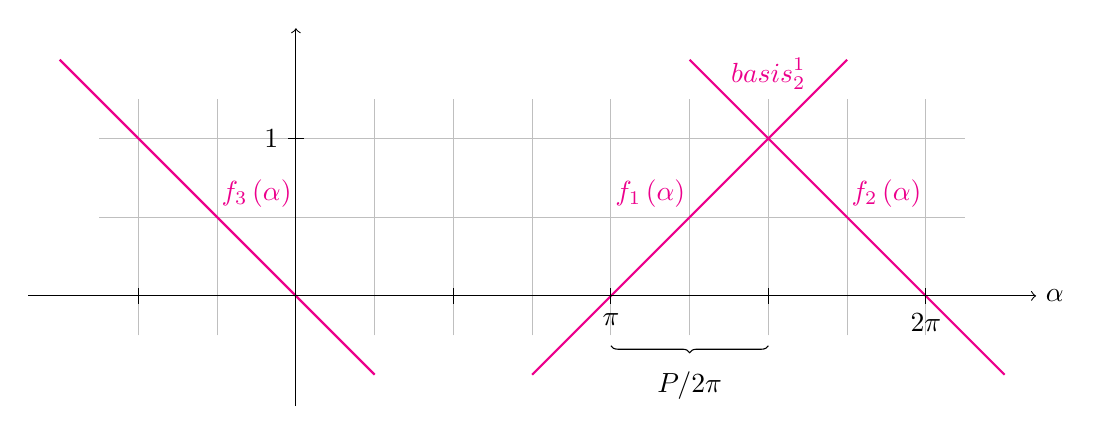
\begin{tikzpicture}
  \draw[color=lightgray] (-2.5, -0.5) grid (8.5, 2.5);

  \draw[thick,color=magenta] (3, -1) -- node[shift={(-0.5,0.3)}] {$f_1\left(\alpha\right)$} (7, 3);
  \draw[thick,color=magenta] (9, -1) -- node[shift={(0.5,0.3)}]  {$f_2\left(\alpha\right)$} (5, 3);
  \draw[thick,color=magenta] (1, -1) -- node[shift={(0.5,0.3)}]  {$f_3\left(\alpha\right)$} (-3, 3);

  \draw[->] (-3.4, 0) -- (9.4, 0) node[right] {$\alpha$};
  \draw[->] (0, -1.4) -- (0, 3.4);
  \draw (0.1, 2) -- (-0.1, 2) node[left] {$1$};
  \draw (-2, 0.1) -- (-2, -0.1);
  \draw (2, 0.1) -- (2, -0.1);
  \draw (4, 0.1) -- (4, -0.1) node[below] {$\pi$};
  \draw (6, 0.1) -- (6, -0.1);
  \draw (8, 0.1) -- (8, -0.1) node[below] {$2\pi$};

  \draw[color=magenta] (6,2.5) node[above] {$\gls{basis}_2^1$};

  \draw [decoration={brace,mirror,raise=18pt},decorate] (4,0) -- node[below=24pt] {$P/2\pi$} (6,0);

\end{tikzpicture}
\caption[Geschlossene B-Spline-Basisfunktionen]{}
\label{fig:bspline_beweis}
\end{figure}
